\documentclass[tikz,border=12pt]{standalone}
\usepackage[T1]{fontenc}
\usepackage{mathpazo}
\usepackage{amsmath,amssymb}
\usetikzlibrary{arrows.meta, calc}

\definecolor{stblue}{HTML}{7B97AD}
\definecolor{rwgold}{HTML}{B8995E}
\definecolor{sage}{HTML}{7A9A7E}
\definecolor{dkbrown}{HTML}{3D3530}
\definecolor{wmgray}{HTML}{7B7067}
\definecolor{cream}{HTML}{F9F6F0}
\definecolor{border}{HTML}{D4C9B8}
\definecolor{terracotta}{HTML}{C47A6A}
\definecolor{lavender}{HTML}{907EA0}

\begin{document}
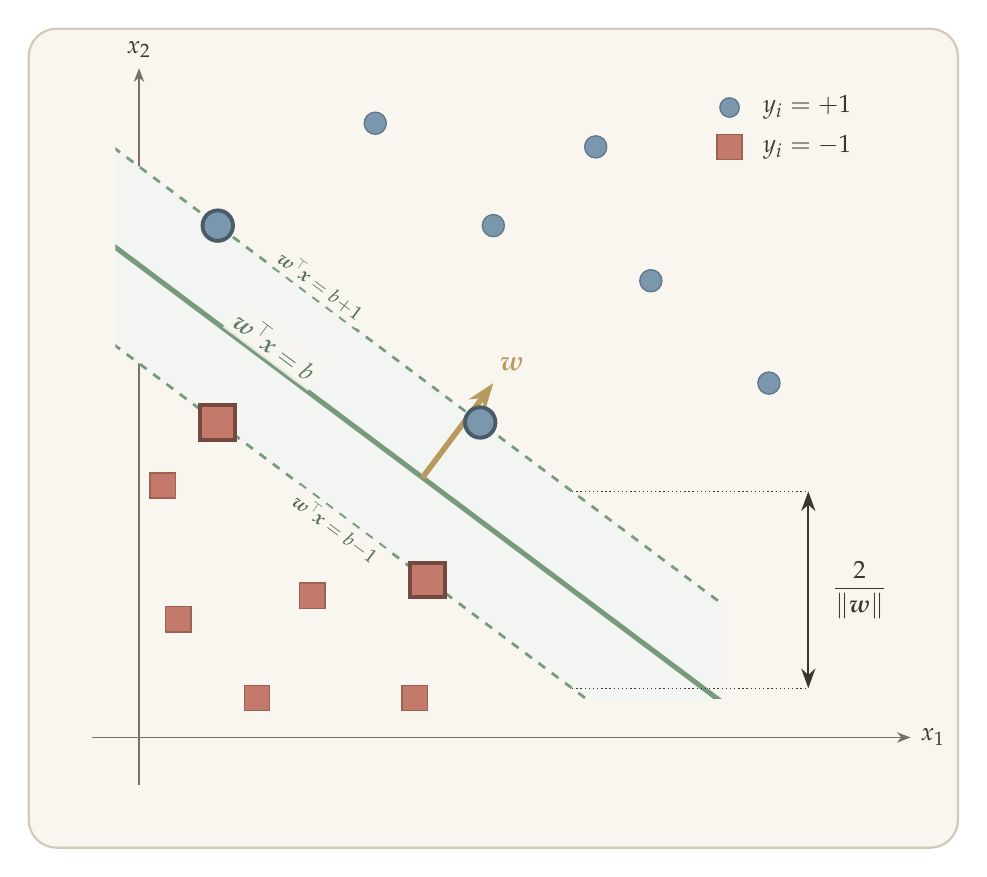
\begin{tikzpicture}[
  >={Stealth[length=3.5mm, width=2.5mm]},
  axis/.style={-{Stealth[length=5pt]}, wmgray, line width=0.6pt},
  lbl/.style={dkbrown, font=\small},
]

% ══════════════════════════════════════════════════════
% Geometry
% ══════════════════════════════════════════════════════
% Hyperplane:  0.75*x1 + x2 = 6.0
%   Normal: (0.75, 1),  ||w|| = 1.25
%   Perpendicular half-margin = 1.0
% Upper margin: 0.75*x1 + x2 = 7.25  (class +1 boundary)
% Lower margin: 0.75*x1 + x2 = 4.75  (class -1 boundary)

\pgfmathsetmacro{\wnx}{0.6}    % 0.75/1.25
\pgfmathsetmacro{\wny}{0.8}    % 1.0/1.25
\pgfmathsetmacro{\rotang}{-36.87}

% Shared clip for shading and lines
\newcommand{\marginclip}{(-0.3, 0.5) rectangle (7.4, 7.5)}

% ══════════════════════════════════════════════════════
% Background
% ══════════════════════════════════════════════════════
\fill[cream, rounded corners=10pt] (-1.4,-1.4) rectangle (10.4,9.0);
\draw[border, line width=0.8pt, rounded corners=10pt]
  (-1.4,-1.4) rectangle (10.4,9.0);

% ══════════════════════════════════════════════════════
% Axes
% ══════════════════════════════════════════════════════
\draw[axis] (-0.6,0) -- (9.8,0) node[right, lbl] {$x_1$};
\draw[axis] (0,-0.6) -- (0,8.5) node[above, lbl] {$x_2$};

% ══════════════════════════════════════════════════════
% Margin shading
% ══════════════════════════════════════════════════════
\begin{scope}
  \clip \marginclip;
  \fill[sage!10]
    (-1, {4.75+0.75}) -- ({(4.75+1)/0.75}, -1)
    -- ({(7.25+1)/0.75}, -1) -- (-1, {7.25+0.75}) -- cycle;
\end{scope}

% ══════════════════════════════════════════════════════
% Three parallel lines
% ══════════════════════════════════════════════════════
\begin{scope}
  \clip \marginclip;

  % Lower margin: 0.75*x1 + x2 = 4.75
  \draw[sage, dashed, line width=1pt]
    (-1, {4.75+0.75}) -- ({(4.75+1)/0.75}, -1);

  % Hyperplane: 0.75*x1 + x2 = 6.0
  \draw[sage, line width=1.8pt]
    (-1, {6.0+0.75}) -- ({(6.0+1)/0.75}, -1);

  % Upper margin: 0.75*x1 + x2 = 7.25
  \draw[sage, dashed, line width=1pt]
    (-1, {7.25+0.75}) -- ({(7.25+1)/0.75}, -1);
\end{scope}

% ══════════════════════════════════════════════════════
% Normal vector w
% ══════════════════════════════════════════════════════
% On hyperplane at x1=3.6: x2 = 6.0-2.7 = 3.3
\coordinate (wbase) at (3.6, 3.3);
\draw[->, rwgold, line width=2pt]
  (wbase) -- ($(wbase) + 1.5*(\wnx, \wny)$)
  node[rwgold, font=\normalsize, anchor=south west, xshift=-2pt]
  {$\boldsymbol{w}$};

% ══════════════════════════════════════════════════════
% Margin annotation: perpendicular double-arrow in clear
% space on the right, between the two dashed lines
% ══════════════════════════════════════════════════════
% The key: place it at a point where both margin boundaries
% are visible and there's no data nearby.
% At x1=6.8, the hyperplane gives x2 = 6.0 - 5.1 = 0.9
% Upper margin: x2 = 7.25 - 5.1 = 2.15
% Lower margin: x2 = 4.75 - 5.1 = -0.35 (below axis)
%
% Instead, use a right-side callout:
% Draw two short horizontal lines from the margin boundaries
% to the right margin of the figure, then a vertical double-arrow.

% Points where margin lines exit the clip at x1=7.4:
% Upper: x2 = 7.25 - 0.75*7.4 = 1.7
% Lower: x2 = 4.75 - 0.75*7.4 = -0.8 (off screen)
%
% Use x1=5.5 instead:
% Upper: x2 = 7.25 - 4.125 = 3.125
% Lower: x2 = 4.75 - 4.125 = 0.625
% Hyperplane: x2 = 6.0 - 4.125 = 1.875
% Both visible, good clear area to the right of SV at (3.67, 2.0)

% Horizontal leader lines from margin boundaries at x1=5.5
% to a vertical arrow at x1=8.5
\pgfmathsetmacro{\annx}{5.5}
\pgfmathsetmacro{\annUy}{7.25 - 0.75*\annx}  % 3.125
\pgfmathsetmacro{\annLy}{4.75 - 0.75*\annx}  % 0.625
\pgfmathsetmacro{\arrx}{8.5}

% Horizontal dashed leader lines
\draw[dkbrown, line width=0.5pt, densely dotted]
  (\annx, \annUy) -- (\arrx, \annUy);
\draw[dkbrown, line width=0.5pt, densely dotted]
  (\annx, \annLy) -- (\arrx, \annLy);

% Vertical double-headed arrow
\draw[{Stealth[length=2.5mm, width=1.8mm]}-{Stealth[length=2.5mm, width=1.8mm]},
      dkbrown, line width=0.8pt]
  (\arrx, \annLy) -- (\arrx, \annUy);

% Label next to the arrow
\pgfmathsetmacro{\annMy}{(\annUy + \annLy)/2}  % 1.875
\node[dkbrown, font=\small, anchor=west, xshift=5pt]
  at (\arrx, \annMy)
  {$\dfrac{2}{\|\boldsymbol{w}\|}$};

% ══════════════════════════════════════════════════════
% Class +1 data (blue circles)
% ══════════════════════════════════════════════════════
\foreach \px/\py in {%
  3.0/7.8, 4.5/6.5, 5.8/7.5, 6.5/5.8, 8.0/4.5%
}{
  \fill[stblue] (\px, \py) circle (4pt);
  \draw[stblue!80!black, line width=0.5pt] (\px, \py) circle (4pt);
}

% Support vectors on upper margin: 0.75*x1 + x2 = 7.25
\pgfmathsetmacro{\svbx}{13/3}
\foreach \px/\py in {1.0/6.5, \svbx/4.0}{
  \fill[stblue] (\px, \py) circle (5.5pt);
  \draw[stblue!60!black, line width=1.4pt] (\px, \py) circle (5.5pt);
}

% ══════════════════════════════════════════════════════
% Class -1 data (terracotta squares)
% ══════════════════════════════════════════════════════
\foreach \px/\py in {%
  0.5/1.5, 1.5/0.5, 0.3/3.2, 2.2/1.8, 3.5/0.5%
}{
  \fill[terracotta] (\px-0.16, \py-0.16) rectangle ++(0.32, 0.32);
  \draw[terracotta!80!black, line width=0.5pt]
    (\px-0.16, \py-0.16) rectangle ++(0.32, 0.32);
}

% Support vectors on lower margin: 0.75*x1 + x2 = 4.75
\pgfmathsetmacro{\svdx}{11/3}
\foreach \px/\py in {1.0/4.0, \svdx/2.0}{
  \fill[terracotta] (\px-0.22, \py-0.22) rectangle ++(0.44, 0.44);
  \draw[terracotta!60!black, line width=1.4pt]
    (\px-0.22, \py-0.22) rectangle ++(0.44, 0.44);
}

% ══════════════════════════════════════════════════════
% Line labels
% ══════════════════════════════════════════════════════

% Hyperplane label
\node[sage!80!black, font=\small, rotate=\rotang, anchor=south,
      inner sep=2pt, fill=cream, fill opacity=0.85, text opacity=1]
  at (1.6, 4.8) {$\boldsymbol{w}^\top\!\boldsymbol{x} = b$};

% Upper margin label
\node[sage!70!black, font=\scriptsize, rotate=\rotang, anchor=south,
      inner sep=1.5pt, fill=cream, fill opacity=0.85, text opacity=1]
  at (2.2, 5.6) {$\boldsymbol{w}^\top\!\boldsymbol{x} = b\!+\!1$};

% Lower margin label
\node[sage!70!black, font=\scriptsize, rotate=\rotang, anchor=north,
      inner sep=1.5pt, fill=cream, fill opacity=0.85, text opacity=1]
  at (2.6, 2.8) {$\boldsymbol{w}^\top\!\boldsymbol{x} = b\!-\!1$};

% ══════════════════════════════════════════════════════
% Legend
% ══════════════════════════════════════════════════════
\fill[stblue] (7.5, 8.0) circle (3.5pt);
\draw[stblue!80!black, line width=0.5pt] (7.5, 8.0) circle (3.5pt);
\node[dkbrown, font=\small, anchor=west] at (7.8, 8.0) {$y_i = +1$};

\fill[terracotta] (7.34, 7.34) rectangle ++(0.32, 0.32);
\draw[terracotta!80!black, line width=0.5pt]
  (7.34, 7.34) rectangle ++(0.32, 0.32);
\node[dkbrown, font=\small, anchor=west] at (7.8, 7.5) {$y_i = -1$};

\end{tikzpicture}
\end{document}
